%%%%%%%%%%%%%%%%%%%%%%%%%%%%%%%%%%%%%%%%%
% DOCUMENTACION PASANTIA EN SONDA URUGUAY
% ING. JUAN BRAGA
% MAESTRÍA EN INGENIERÍA ELÉCTRICA, UDELAR
% JUNIO 2016
%%%%%%%%%%%%%%%%%%%%%%%%%%%%%%%%%%%%%%%%%

%----------------------------------------------------------------------------------------
%	PACKAGES AND DOCUMENT CONFIGURATIONS
%----------------------------------------------------------------------------------------

\documentclass{article}

\usepackage[version=3]{mhchem} % Package for chemical equation typesetting
\usepackage{siunitx} % Provides the \SI{}{} and \si{} command for typesetting SI units

\usepackage[spanish]{babel}
\selectlanguage{spanish}
\usepackage[utf8]{inputenc}
\usepackage{graphicx} % Required for the inclusion of images
\usepackage{natbib} % Required to change bibliography style to APA
\usepackage{amsmath} % Required for some math elements 

\setlength\parindent{0pt} % Removes all indentation from paragraphs

\renewcommand{\labelenumi}{\alph{enumi}.} % Make numbering in the enumerate environment by letter rather than number (e.g. section 6)

%\usepackage{times} % Uncomment to use the Times New Roman font

%----------------------------------------------------------------------------------------
%	DOCUMENT INFORMATION
%----------------------------------------------------------------------------------------

\title{\textbf{Desarrollo de una plataforma de procesamiento de audio en tiempo real con aplicación a seguridad urbana}\\ \textsc{Pasantía Laboral en SONDA Uruguay}\\
\large \textsc{Maestría en Ingeniería Eléctrica} del \textit{Instituto de Ingeniería Eléctrica, Facultad de Ingeniería, Universidad de la República, Uruguay.}}

\author{\textit{Ing. Juan Braga}}
\date{\today}

\begin{document}

\maketitle 

\begin{center}
\begin{tabular}{l r}
\medskip
\textsc{Período:} & \textsc{Diciembre 2015 a Marzo 2016}\\ % Date the experiment was performed
\textsc{Docente Responsable:} & \textit{Msc. Ing. Guillermo Carbajal} \\ 
\textsc{Responsable SONDA Uruguay:} & \textit{Nestor Rossi}, Gerente de Proyectos  \\
\textsc{Equipo de SONDA Uruguay:} & \textit{Ing. Florencia Lanzaro} \\ & \textit{Msc. Ing. Guillermo Carbajal} \\ 
\end{tabular}
\end{center}

%----------------------------------------------------------------------------------------
%	ABSTRACT
%----------------------------------------------------------------------------------------

\begin{abstract}
El presente informe tiene como objetivo la documentación del trabajo realizado en SONDA Uruguay en el período de Diciembre 2015 a Marzo 2016 para su aprobación en créditos de la Maestría en Ingeniería Eléctrica de la UdelaR. Se trató de un estudio del estado del arte sobre la aplicación de analíticas a seguridad urbana y el desarrollo de una plataforma de procesamiento de audio en tiempo real para prueba de concepto en condiciones de laboratorio. En lo que sigue se detalla sobre el desarrollo realizado así como los algoritmos utilizados, con referencias a publicaciones científicas, para la implementación de dos analíticas de audio en particular. 
\end{abstract}

%----------------------------------------------------------------------------------------
%	SECTION 1
%----------------------------------------------------------------------------------------

\section{Introducción}
El monitoreo en tiempo real de las actividades humanas para seguridad urbana se ha vuelto masivo en los últimos años a nivel mundial. La cantidad de sensores distribuidos por las ciudades ha crecido enormemente. Es entonces en los centros de monitoreo, donde confluyen las señales desde variados puntos de la ciudad, que surge la necesidad de automatizar los procesos de visualización y control para hacer la operativa más eficiente \citep{Crocco:2016:ASS:2891449.2871183}. El desarrollo de analíticas en tiempo real para detección automática de patrones de interés, ha captado la atención de la comunidad científica así como a empresas con fines comerciales. En este escenario es donde la empresa SONDA Uruguay motiva un proyecto de desarrollo de software de analíticas de audio y video, para el monitoreo automático en tiempo real de los espacios urbanos.  

\smallskip
En el marco del proyecto de la empresa anteriormente mencionado, se realizó una prueba de concepto sobre la implementación de analíticas de audio en tiempo real para seguridad urbana. Con este fin se realizó un estudio del estado del arte para luego seguir con el desarrollo de una plataforma de procesamiento de audio a nivel de laboratorio. 

\smallskip
En lo que sigue el documento está dividido en tres secciones. En la Sección \ref{PP} se detalla sobre la plataforma de procesamiento desarrollada. En la Sección \ref{analiticas} los algoritmos utilizados para la implementación de dos analíticas de audio particulares: Detección de Niveles Predefinidos de Sonido y Detección de Sirenas. Por último en la Sección \ref{concl} una breve reflexión sobre la sinergia de la pasantía laboral y los estudios de académicos principalmente el tema de tesis, en el marco de la Maestría de Ingeniería Eléctrica actualmente en curso.  

\subsection{Sobre SONDA Uruguay}
SONDA Uruguay es fundamentalmente una empresa de servicios, proyectos de integración de sistemas y provisión de plataformas en el campo de las tecnologías de la información. Actualmente la empresa está incorporando proyectos de I+D en el área de tratamiento de señales. Tal es el caso del proyecto de desarrollo de analíticas de audio y video en tiempo real con aplicación a seguridad urbana. En el mismo, se encuentran involucradas ocho personas, profesionales y estudiantes de Ingeniería de Sistemas y Eléctrica, que complementan la rama de computación científica con el manejo de la ingeniería de software para aplicaciones críticas de gran volumen de datos.  

\subsection{Sobre el grado de avance del proyecto}                            
Al día de hoy el software de analíticas forma parte de la tecnología implantada en el Centro de Monitoreo (CM) del Ministerio del Interior, en el proyecto Ciudad Segura. La versión actual cuenta únicamente con analíticas basadas en el procesamiento de la señal de video. Es utilizado para apoyar la operativa de los visualizadores del CM, alertando automáticamente frente a eventos de interés predefinidos, mediante el procesamiento de señales en tiempo real.  


%----------------------------------------------------------------------------------------
%	SECTION 2
%----------------------------------------------------------------------------------------

\section{Plataforma de procesamiento}
\label{PP}
Los sensores para Seguridad Urbana (en particular las cámaras de video y micrófonos) son diseñados para trabajar en tiempo real, transmitiendo a través de una red IP los datos adquiridos, a una central donde se realiza el monitoreo y la toma de decisiones. Es en este escenario donde los algoritmos de procesamiento de audio se encuentran embebidos y los tiempos de procesamiento no deben exceder la cadencia de disponibilidad de datos.

\smallskip
La plataforma de procesamiento, se puede dividir en dos grandes bloques: por un lado el de genereración de datos de audio y comunicaciones, y por otro la adquisición desde la red y procesamiento para la toma de decisiones, como se observa en la Figura \ref{fig:plataforma_procesamiento}.
\smallskip

Del lado de la generación de los datos de audio el tipo de micrófono (patrón polar, sensibilidad, etc.) y el codec (frecuencia de muestreo, bitdepth, etc.) a utilizar definen la información sonora que se extrae del escenario monitoreado El tipo de análisis que se pueda hacer va a depender entonces de estos dos bloques.
\smallskip

El módulo de adquisición hace disponible las muestras de audio, en ventanas de largo configurable según los requerimientos del algoritmo. El análisis se hace ventana a ventana (frame by frame en la literatura) y en el caso particular de detección de sirenas (sección: \ref{deteccion de sirenas}), se utiliza una estrategia de integración temporal para aumentar la robustez a falsas alarmas, debidas al análisis local ventana a ventana.


\begin{figure}[h]
\begin{center}

\includegraphics[width=0.65\textwidth]{plataforma_procesamiento} 
\caption{Esquema de la plataforma de procesamiento. A la izquierda el bloque de generación y comunicaciones, a la derecha el de adquisición y procesamiento.}
\label{fig:plataforma_procesamiento}
\end{center}
\end{figure}

%----------------------------------------------------------------------------------------
%	SECTION 3
%----------------------------------------------------------------------------------------

\section{Analíticas}
\label{analiticas}
Las analíticas son el modulo de procesamiento de audio que transforman los datos de entrada en una decisión para generar una alarma. Tienen el objetivo de alertar a los operadores del CM ante hechos predefinidos que puedan estar asociados a actividades vandálicas. En esta sección se describe sobre dos analíticas desarrolladas en la primer etapa del proyecto de desarrollo del software de analíticas de audio. 

\subsection{Analítica de Detección de Niveles Predefinidos de Sonido}
Tiene como objetivo alertar la presencia de momentos de alto nivel sonoro o ausencia del mismo. Se hace una estimación de la energía, de la señal de entrada, frame a frame y se umbraliza para generar alertas en niveles energéticos predefinidos por el usuario.

\subsubsection{Medidas de energía utilizadas}
Se utilizan dos estimaciones de energía para detección de cambios energéticos de distinta naturaleza, por un lado cambios sostenidos en el tiempo y por otro lado los impulsivos.

\subsubsection*{RMS}
Se utiliza para estimar la energía promedio de la ventana temporal. La ecuación para una ventana de largo N es de la siguiente forma \cite[Chapter~4]{Lerch:2012:IAC:2392638}:
\begin{equation}
RMS = \sqrt{\frac{1}{N}\sum_{n=1}^{N} x[n]^2}
\end{equation}

\subsubsection*{Envolvente de pico}
Se utiliza para detectar eventos energéticos impulsivos que pueden ser disimulados por el promediado del valor RMS. El cálculo para una ventana de largo N se realiza de la siguiente forma \cite[Chapter~4]{Lerch:2012:IAC:2392638}:
\begin{equation}
PICO = max(x[n])\forall n \in 1..N 
\end{equation}

\subsubsection{Detección de altos niveles sonoros}
Para esta analítica se utiliza una estrategia de doble umbral sobre las estimaciones de energía detalladas anteriormente. En primer lugar se aplica al valor RMS de la ventana temporal, siendo útil frente a cambios energéticos sostenidos en el tiempo. Por otro lado se umbraliza el valor de pico, para detectar eventos impulsivos que no sean detectables en el promediado del RMS.

\subsubsection{Detección de bajos niveles sonoros}
Para la umbralización inferior sólo se trabaja con el valor RMS.

\subsection{Analítica de Detección de Sirenas}
\label{deteccion de sirenas}
Tiene como objetivo alertar frente a al presencia de una sirena en el audio de análisis. Para esta analítica se utilizó una estrategia de reconocimiento de patrones con el entrenamiento de clasificadores. Se resolvió con el enfoque clásico de reconocimiento de sonidos particulares para Seguridad Urbana de dos etapas, \cite{lecomte2011abnormal}:
\begin{enumerate}
\begin{item}
Detección de eventos anómalos
\end{item}
\begin{item}
Reconocimiento de los eventos anómalos detectados
\end{item}
\end{enumerate}

Se trata de dos clasificadores anidados con una etapa de integración temporal intermedia. En la primer etapa, con un modelado no supervisado del ruido ambiente se detectan anormalidades en el audio, si existieron los suficientes eventos anómalos según la integración temporal, se pasa a la tercer y última etapa, donde se clasifica en sirena o no. Se observa un esquema de lo dicho anteriormente en la Figura \ref{fig:deteccion_sirenas}. 
 
\begin{figure}[h]
\begin{center}
\includegraphics[width=0.8\textwidth]{deteccion_sirenas} 
\caption{Esquema de la analítica de detección de sirenas. Se observa una primer etapa de substracción de fondo y posterior clasificación en sirena o no.}
\label{fig:deteccion_sirenas}
\end{center}
\end{figure}

\subsubsection{Substractor de Fondo}
En aplicaciones de Seguridad Urbana, se utilizan algoritmos de substracción de fondo (en la literatura \textit{Background Substraction}, \cite{Crocco:2016:ASS:2891449.2871183}) como una primer etapa de análisis y conceptualización de la señal de entrada. En otras palabras estos algoritmos modelan los patrones que dominan el ambiente y detectan anormalidades.
\smallskip 

El modelado del ruido ambiente con un enfoque supervisado tiene la dificultad de la generación de una base de datos que resuma y caracterice la infinidad de posibilidades que existen en un entorno urbano. Por esta razón se optó por un enfoque de clase unitaria utilizando One-Class SVM (\cite{rabaoui2008one}, \citep{lecomte2011abnormal}).

\subsubsection*{Extracción de Características}
Teniendo en cuenta que no se conoce nada a priori sobre el ruido ambiente y además el sistema está basado en un análisis por ventana (en la literatura frame by frame), para la extracción de características se utiliza el enfoque genérico de un banco de filtros lineal, para extracción de la energía en bandas de frequencia de la transformada de Fourier (Fourier-based linear filterbank \citep{lecomte2011abnormal}).

\subsubsection*{Entrenamiento y Clasificación}
El entrenamiento se realiza en tiempo real, con fragmentos del propio ruido ambiente en donde el sistema se encuentra funcionando. Permite independencia de una base de datos para entrenamiento y robustez frente a cambios naturales en el escenario de análisis, como son la noche y el día por ejemplo. 
\smallskip

El largo del fragmento es variable permitiendo adaptarse a escenarios complejos, sacrificando costo computacional. Se utiliza un clasificador One-Class SVM que detecta en cada ventana de entrada si pertenece o no al modelo de fondo generado en el One-Class SVM.

\subsubsection{Integración temporal}

Previo a la etapa de clasificación de sirena o no, se utiliza un esquema de integración temporal y una medida de distancia para decidir si continuar o descartar las muestras de audio.

\smallskip
Se integran ventanas adyacentes y mediante la distancia binaria de Huffman, con un umbral parametrizable, se define si ese fragmento mayor de audio pasa a la siguiente etapa de clasificación, observar Figura \ref{fig:integracion_temporal}. 

\begin{figure}[h]
\begin{center}
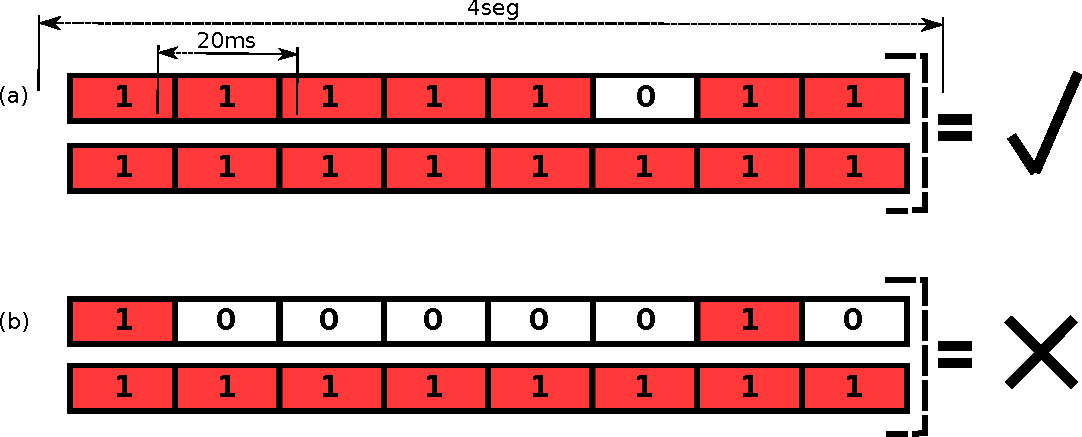
\includegraphics[width=0.9\textwidth]{integracion_temporal} 
\caption{Esquema de la integración temporal de ventanas adyacentes en un fragmento de audio mayor, se ejemplifica con dos valores particulares en segundos. En verde los audios detectados como no fondo, en blanco los que pertenecen al fondo según el substractor de fondo. En (a) se observa un audio que pasa a la segunda etapa de clasificación, en (b) caso contrario.}
\label{fig:integracion_temporal}
\end{center}
\end{figure}
 
\subsubsection{Clasificación Sirena}
La última etapa es un clasificador One-Class SVM que decide si el evento anómalo sostenido en el tiempo, según las etapas anteriores, clasifica como sirena o no. 

\subsubsection*{Extracción de Características}
Se utilizan al igual que en la publicación \cite{Salamon:UrbanSound:ACMMM:14} los primeros 25 coeficientes MFCC (Mel-Frequency Cepstral Coeficients), calculados sobre un banco de filtros Mel de 40 bandas, generado con ventanas temporales de 20ms, 50\% de solapamiento y enventanado hamming. Lo anterior se computa sobre el audio completo que sale de la integración temporal (en la Figura \ref{fig:integracion_temporal} se ejemplifica con 4 segundos de audio) y se aplican estadísticas para resumir a un vector de 275 características: máximo, mínimo, media, mediana, varianza, skewness, kurtosis y media y varianza de la primer y segunda derivada de los coeficientes Mel a lo largo del tiempo.

\subsubsection*{Entrenamiento y Clasificación}
Para el entrenamiento se utilizó un enfoque de clase unitaria utilizando One-Class SVM. Para la base de datos se utilizaron audios recopilados de internet y algunas grabaciones hechas en el ambiente de laboratorio y en la calle. 

%----------------------------------------------------------------------------------------
%	SECTION 4
%----------------------------------------------------------------------------------------

\section{Conclusiones}
\label{concl}
La pasantía laboral generó sinergia de mis estudios académicos y mi trabajo en el sector privado. El desarrollo de analíticas de audio requiere de habilidades en procesamiento de audio que están vinculadas directamente con mi tema de tesis. Además se procedió con metodologías y herramientas aprendidas en la Maestría en Ingeniería Eléctrica de la Facultad de Ingeniería, como la realización de una revisión bibliográfica de publicaciones científicas para dominar el estado del arte, y la utilización de herramientas vistas en cursos de la maestría.
\smallskip

Por otro lado la posibilidad de aplicar directamente los conocimientos obtenidos en la Maestría de Ingeniería Eléctrica a la resolución de un problema particular con aplicación práctica, generó motivación tanto para los estudios académicos como para mi rol como ingeniero en la sociedad.  

%----------------------------------------------------------------------------------------
%	BIBLIOGRAPHY
%----------------------------------------------------------------------------------------


\newpage
\bibliographystyle{apalike}
\bibliography{sample}

%----------------------------------------------------------------------------------------
\end{document}
